\usepackage{multirow}
\usepackage{subfigure}  % use for side-by-side figures

\section{Trigger requirements}
\label{sc:TriggerRequirements}

Events analyzed in this note were collected by the CMS experiment during the LHC
commissioning phase in December 2009. The majority of collisions
recorded in this period were at $\sqrt{s}=900$~GeV, and a
smaller dataset was collected with $\sqrt{s}=2.36$~TeV. In order to
identify the collision candidates, we use the following
set of Level-1 ``technical'' triggers (TT), which are based on the Beam Scintillation
Counter (BSC) system:

\begin{itemize}
\item At least one of the BSC MinBias TT: require that at least one of
  the TT bits 40 or 41 fired. These triggers fire when there is a
  coincident activity in the forward and backward BSC detectors,
  indicating a collision candidate. Events collected by this triggers are found in the Minimum Bias dataset.

\item None of the BSC beam halo triggers fired: exclude events where any
  of TT bits 36, 37, 38, 39 fired. These triggers fire when the hits in
  the forward and backward BSC detectors are inconsistent in timing with
  originating from the collision.
\end{itemize}

\section{Data Samples}
\label{sc:DataSamples}

The events collected by the BSC MinBias TT bits 40 and 41 can be found
in ``MinimumBias'' dataset. For the analysis presented in this note the
collision events were reconstructed using CMSSW\_3\_3\_5\_patch4
software release. We used the data sample in which trigger selections
discussed in the previous section are already applied:
\begin{itemize}
\item
  /MinimumBias/BeamCommissioning09-BSCNOBEAMHALO-Dec14thSkim\_v1/RAW-RECO
\end{itemize}
Additionally, we require that L1 TT bit 0 was fired, which
indicates consistent timing with LHC bunch crossing. We also require
that the ``HLT\_PhysicsDeclared'' bit is set, which indicates that all
CMS systems were up and running with stable beams in the
accelerator. 

Out of all runs present in this data set that fulfill all
of the requirements listed above, the following runs were identified by the
JetMET DQM, ECAL/HCAL DPG groups to have
calorimeter problems (``bad'' runs): 123970, 123976, 123977, 123978, 123985, 123987,
124006. Events collected during these runs are excluded
from this analysis, unless it is stated otherwise.

After excluding the bad runs listed above, the following set of runs is
used for the analysis presented in this note:
\begin{itemize}
\item For the $\sqrt{s}=900$~GeV data-taking period:
123815, 123818, 123906, 123908, 123909, 123970, 123976, 123977, 123978,
123985, 123987, 124006, 124008, 124009, 124017, 124020, 124022, 124023,
124024, 124025, 124027, 124030. 

\item For the $\sqrt{s}=2.36$~TeV data-taking period: 124120.

\end{itemize}

\subsection{Monte Carlo simulation}

The collision data events considered in this analysis are compared with
{\sc pythia} simulations of Minimum Bias collisions which are processed
with {\sc GEANT-4} simulation of the CMS detector. Simulated events are
then reconstructed using CMSSW\_3\_3\_5\_patch2. The data samples used in
this analysis can be found at:
\begin{itemize}
\item Comparisons with 900~GeV data: /MinBias/Summer09-STARTUP3X\_V8I\_900GeV-v2/GEN-SIM-RECO
\item Comparisons with 2.36~TeV data: /MinBias/Summer09-STARTUP3X\_V8D\_2360GeV-v2/GEN-SIM-RECO
\end{itemize}

For the comparisons of data with Monte Carlo we require that simulated
events pass the BSC Minimum Bias trigger selections (TT bits 40 and
41). Additionally, any further event selection criteria described in the next section
are applied to both data and simulation.

\section{Event Selection}
In order to study the $\etmiss$ performance, an
event selection that removes the instrumental or beam related noise
sources is required. In this section we describe the selection criteria
we use to remove these type of events, and summarize their effect on
$\etmiss$ performance.

% \subsection{Vertex selection}
% In order to further constrain the event selection to identify the
% collision events, several studies have considered a selection based on
% the reconstructed primary vertex properties, such as $Z$ position or
% number of tracks attached to the vertex. The comparison of the vertex
% $Z$ distribution in data compared to simulation is shown on
% Fig.\ref{fig:vertex_selection_1}. Events shown in
% Fig.\ref{fig:vertex_selection_1}  are required to have at least 2 tracks
% attached to the primary vertex. As can be seen from this comparison,
% the simulation does not agree well with the observed distribution of
% this variable. Therefore, we choose not to make any selection on this variable.

% \begin{2figures}{hbtp}
%   \resizebox{8cm}{!}{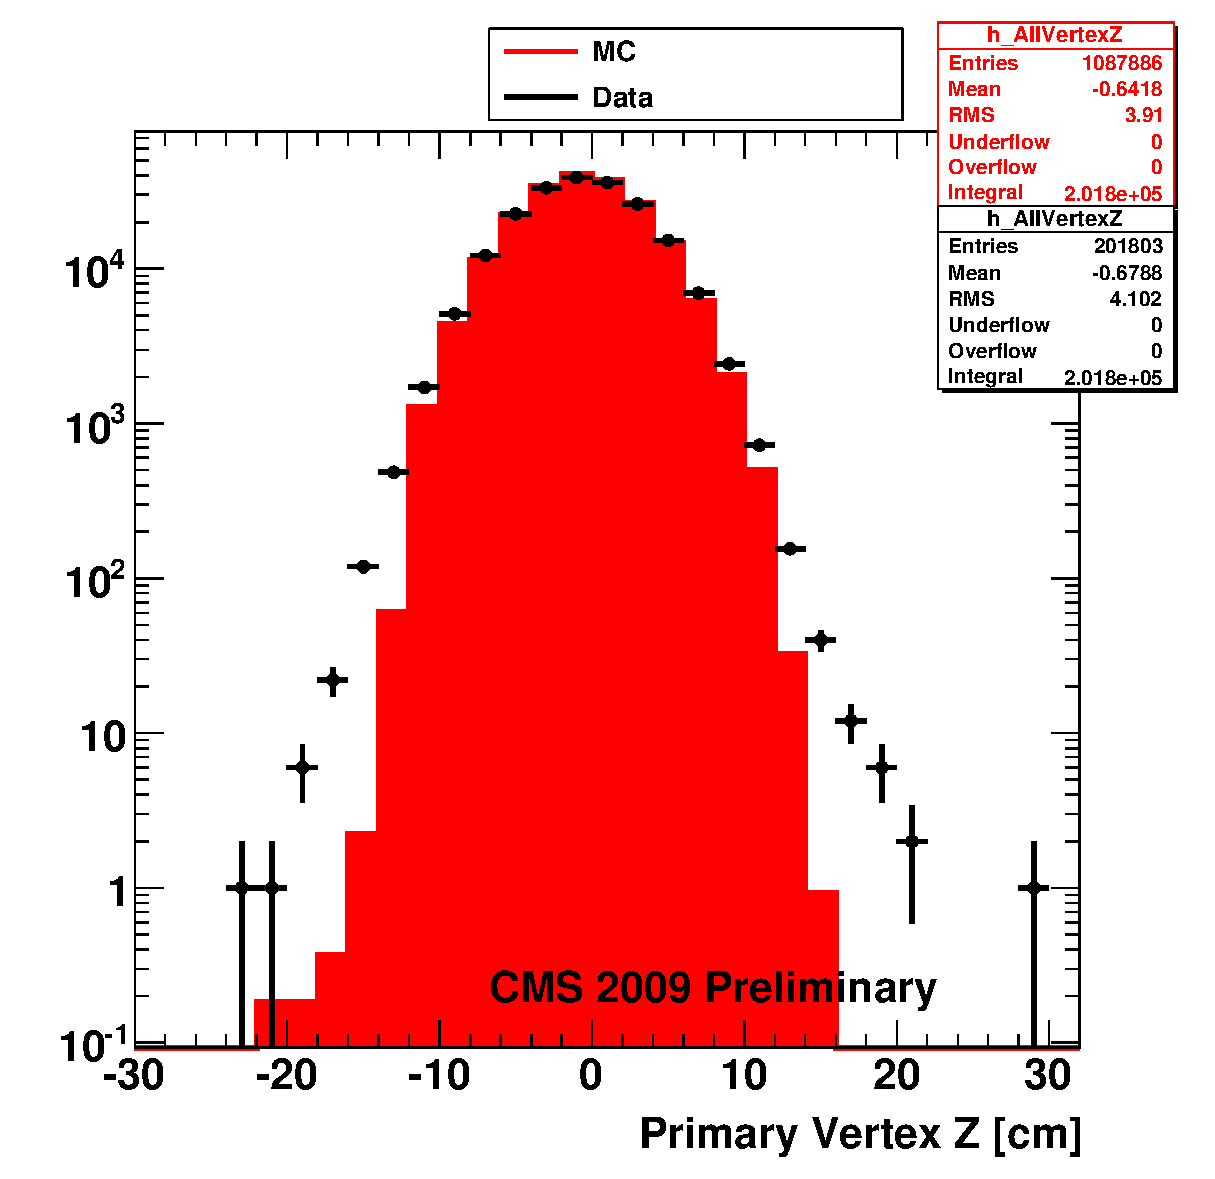
\includegraphics{plots_EventSelection/h_AllVertexZ_log.eps}} &
%   \resizebox{8cm}{!}{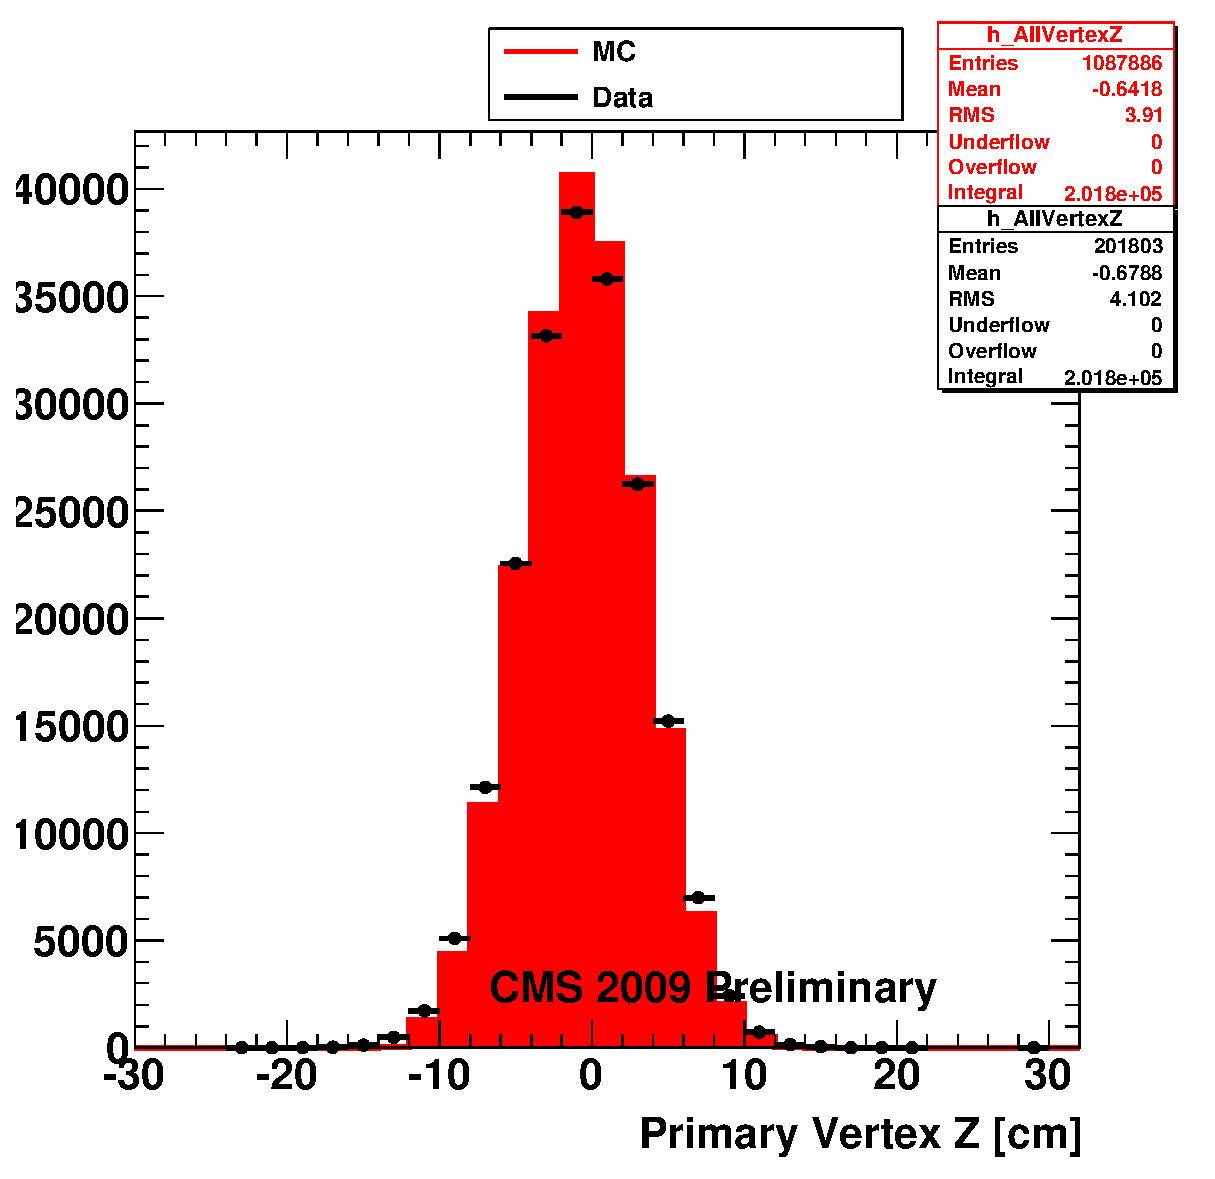
\includegraphics{plots_EventSelection/h_AllVertexZ_linear.eps}} \\
%  \label{fig:vertex_selection_1}
% \caption{Comparison of the distribution of the event primary vertex $Z$
%   position between data and Monte Carlo simulation. Distributions for
%   events that have at least two tracks attached to the vertex are shown.}
% \end{2figures}

\subsection{Removal of scraping events}

During the LHC commissioning phase, it was observed that
in some bunch crossings there was a anomalously large occupancy in the
pixel detector, which resulted in a large number of reconstructed fake
tracks. These events were identified as being the result of beam
particles traversing the pixel detector longitudinally. We reject this
type of events by requiring that the fraction of high-purity tracks in
all events with more than 10 tracks is greater than 20\%.

\subsection{HCAL anomalous noise}
Commissioning studies of the CMS hadronic calorimeter performed 
during past test beam, cosmic, and beam runs have 
identified anomalous noise (i.e. not due to regular 
electronic/pedestal noise) that can grouped in two categories 
(CMS PAPER CFT-09-019):
\begin{itemize}
\item{\bf HB/HE Anomalous Noise} The source of the anomalous noise in the HCAL 
barrel (HB) and endcap (HE) subdetectors is due to characteristics 
of the hybrid photo-diodes (HPDs), used to convert the scintillator light into 
an electrical output, and the readout boxes (RBXs) that they lie within.
Such atypical signals can be categorized 
in i) Ion Feedback Noise (typically affecting 1-2 channels in one HPD), ii) HPD Noise 
(coherent affecting up to 18 channels in one HPD), iii) RBX Noise 
(coherent noise affecting up to 72 channels in one RBX unit);
\item{\bf HF Photo-Multipliers (PMT) Window Hits} An energetic charged particle, directly 
impinging upon the window of an HF PMT, can produce an abnormally large apparent 
energy signal for a single HF channel (the one associated to that PMT). 
\end{itemize}

The presence of such atypical signals was also confirmed in recent 
2009 collision data, sometimes resulting in large unphysical $\etmiss$ in the event. 
Observations indicate that large unphysical HCAL-related $\etmiss$ 
in Minimum Bias events is mostly due to energy reconstructed in HF, 
while in only few cases the energy unbalance is due to HB/HE noise events. 
This can be explained by considering that HF PMT window hits 
are related with the beam activity (i.e. beam halo particles hitting the PMT window), 
while HB/HE noise (HPD and RBX noise) occurs at random time and it is 
uncorrelated with the beam activity. Therefore the probability of overlap 
of an HB/HE noise event with a collision event is small.

The approach used in this note to identify anomalous noise events in HCAL is described below.

\begin{itemize}
%
\item{\bf HBE/HE noise events} A set of algorithms have been developed by the HCAL group to 
identify and address these types of problems in the data. The methods have been tested on cosmic muon data, 
dedicated calorimeter noise data, and single beam data collected at CMS in 2008, 
as described in CMS PAPER CFT-09-019, ADD (link to Twiki page ``HcalNoiseInfoLibrary''). 
Anyway, some of the algorithms for HB/HE noise identification rely on the proper 
timing alignment of the detector, which is not fully understood at the startup.
Therefore, considering also that the probability of overlap between such noise and 
collission events is observed to be very small, it has been decided to follow a conservative approach and 
don't apply any cleaning for HB/HE noise at this stage.
%
\item{\bf HF PMT window hits} PMT windows hits within HF are tagged by comparing 
the energies reconstructed from long (L) and short (S) fibers with the same ($\eta$,$\phi$) values. 
Infact, a particle hitting directly a PMT would produce a large apparent energy only in one channel 
(i.e. either the one connected to long or short fiber) and none in the other.

Given a pair of adjacent long and short fibers at the same ($\eta$,$\phi$) value 
with energies $E^L$, $E^S$, respectively, the fiber channels are flagged as noisy if 
(a) the transverse energy measured in the HF tower ($E_T=E_T^L+E_T^S$) is at least 5~GeV, 
and (b) the energy ratio $R$, defined as:
%
\begin{equation}
R = \frac{E^L - E^S}{E^L + E^S}
\end{equation}
%
is greater than 0.99 (PMT hit associated to the long fiber) 
or smaller than -0.8 (PMT hit associated to the short fiber). 
Figure~\ref{fig:hf_noise_ET_vs_R} shows the scatter distribution of $E_T$ vs $R$, 
for both data and MC, after applying all the event selection criteria except 
the HF filter itself. The HF noise channels can be identified by 
large $E_T$ values and $R$ values close to -1 or 1, 
inconsistent with MinBias MC assumption.

In this study, if at least one HF fiber channel is flagged by this algorithm, 
the event is simply rejected from the analysis. No attempt to clean the event, 
by correcting the high level objects (such as $\etmiss$ or SumET), 
is performed at this stage of the analysis. 
\\
\\
%
%
\begin{figure}[h!]
 \centering
 \begin{tabular}{ll}
  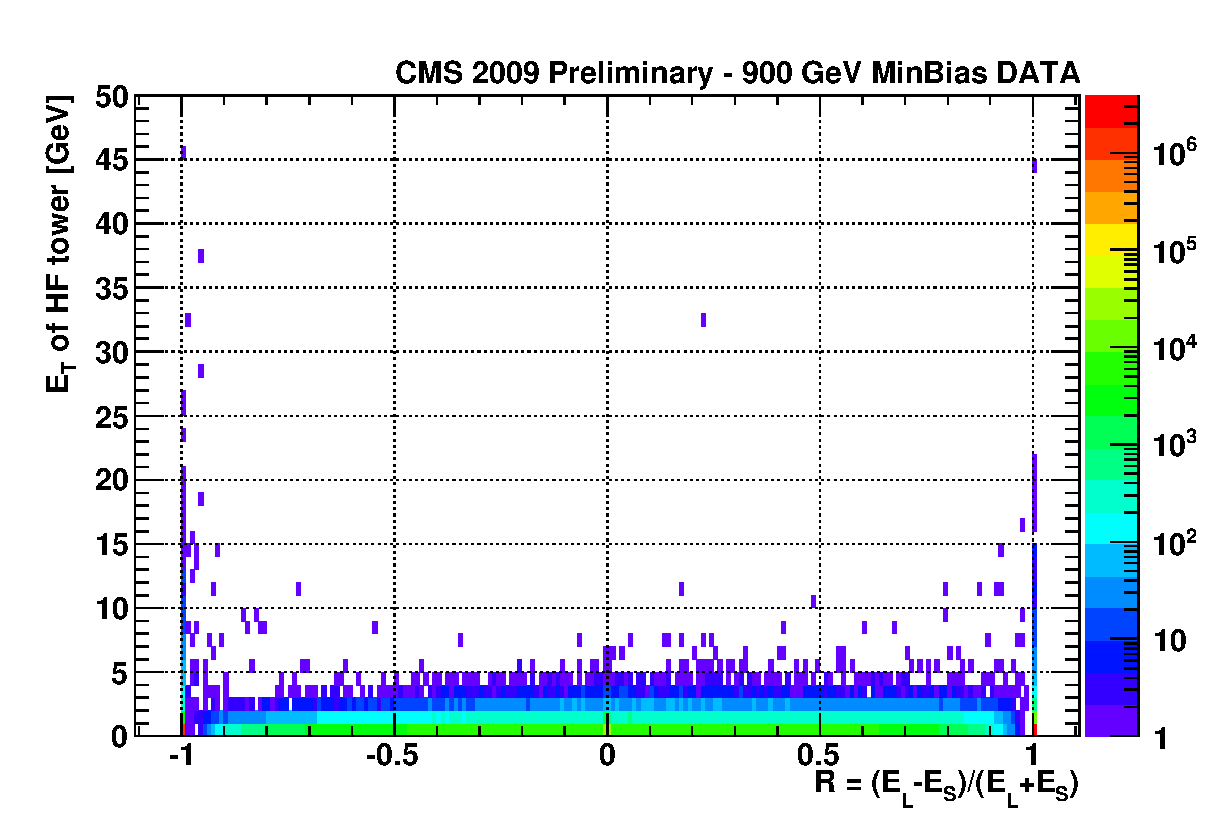
\includegraphics[width=0.5\textwidth]{plots_hcalnoise/hf_towerET_vs_ratio_DATA.eps} &
  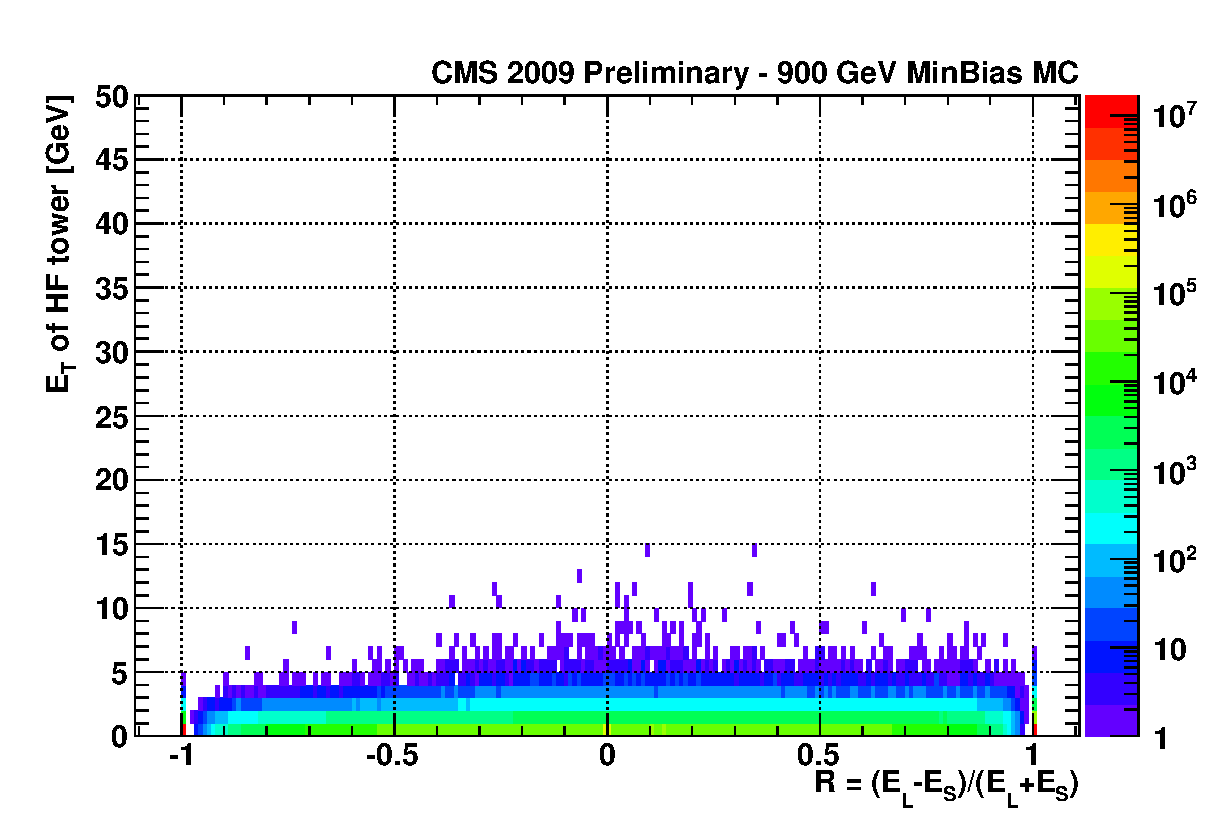
\includegraphics[width=0.5\textwidth]{plots_hcalnoise/hf_towerET_vs_ratio_MC.eps} \\
 \end{tabular}
\caption{\small (Top) Scatter distribution of transverse energy in HF tower versus energy ratio $R$ for both data 
(Left) and MC (Right), after applying all the event selection criteria except the HF filter itself. 
Plots are filled for each HF tower if either $E_L>1.2$~GeV or $E_S>1.8$~GeV (to cut the pedestal noise).
\label{fig:hf_noise_ET_vs_R}}
\end{figure}
%
%
\end{itemize}

\subsection{ECAL anomalous noise}

A set of events with unphysical characteristics in the barrel ECAL
calorimeter was observed during the initial analysis of the
$\sqrt{s}=900$~GeV data collected at CMS. These events are characterized
by energy deposits in a single, isolated ECAL crystal (``spike''
crystal), while the crystals in the immediate neighborhood of the spike
crystal contain little or no energy. This kind of energy deposit is
incompatible with energy deposits due to a real photon or electron,
given the Moliere radius and crystal sizes in ECAL. Since the presence
of a spike crystal in an event with no $\etmiss$ may appear to have
energy imbalance in the transverse plane, it is crucial to identify this
type of noise and efficiently remove it.

Unlike the HCAL anomalous noise described in the previous section, ECAL
spike events were not identified in the data taken before the collision runs
in December 2009 (however, there are indications that spike events may
have been present also before the collision runs). The study to understand the
source of ECAL spike events and to efficiently identify them is
currently ongoing. The approach we have taken to identify the ECAL
spikes in this analysis is described below.

\begin{figure}[h]
 \centering
 \begin{tabular}{ll}
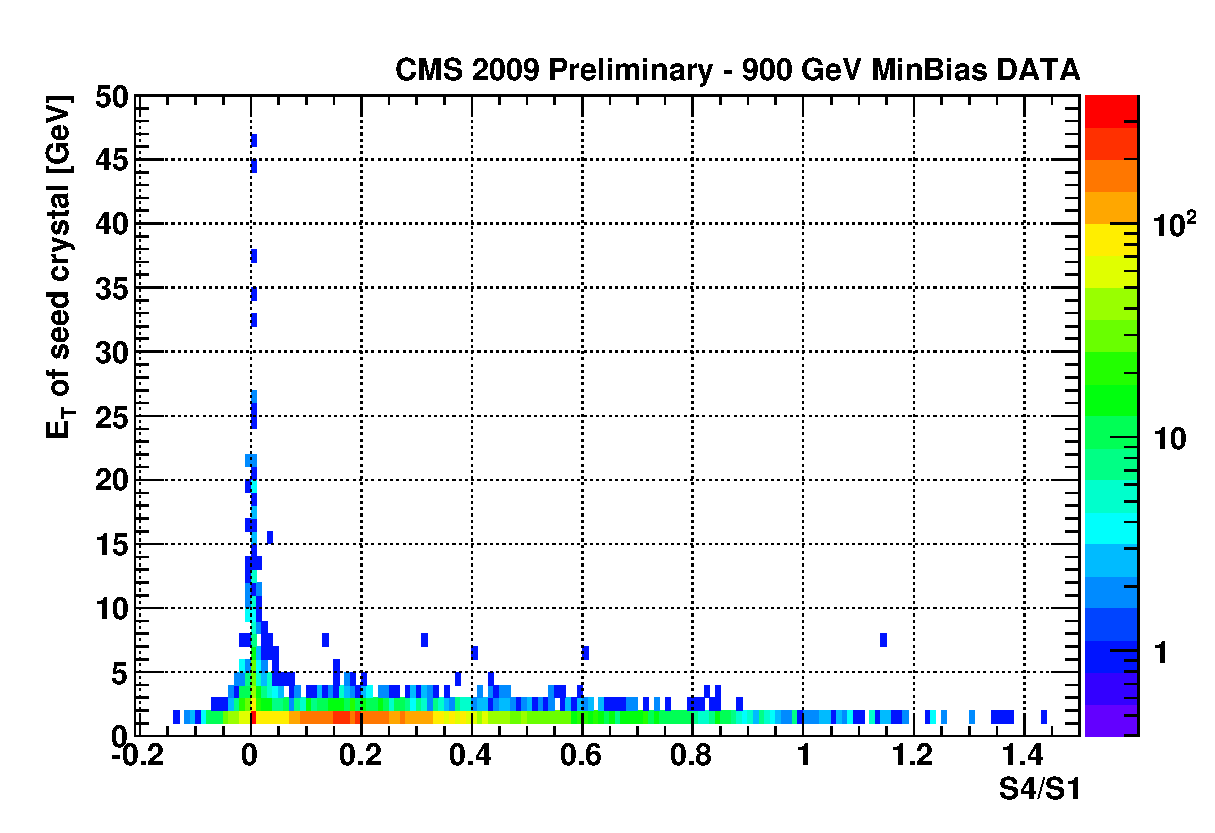
\includegraphics[width=0.5\textwidth]{plots_ecalnoise/ECalSeedET_Vs_S4_DATA900GeV.eps}&
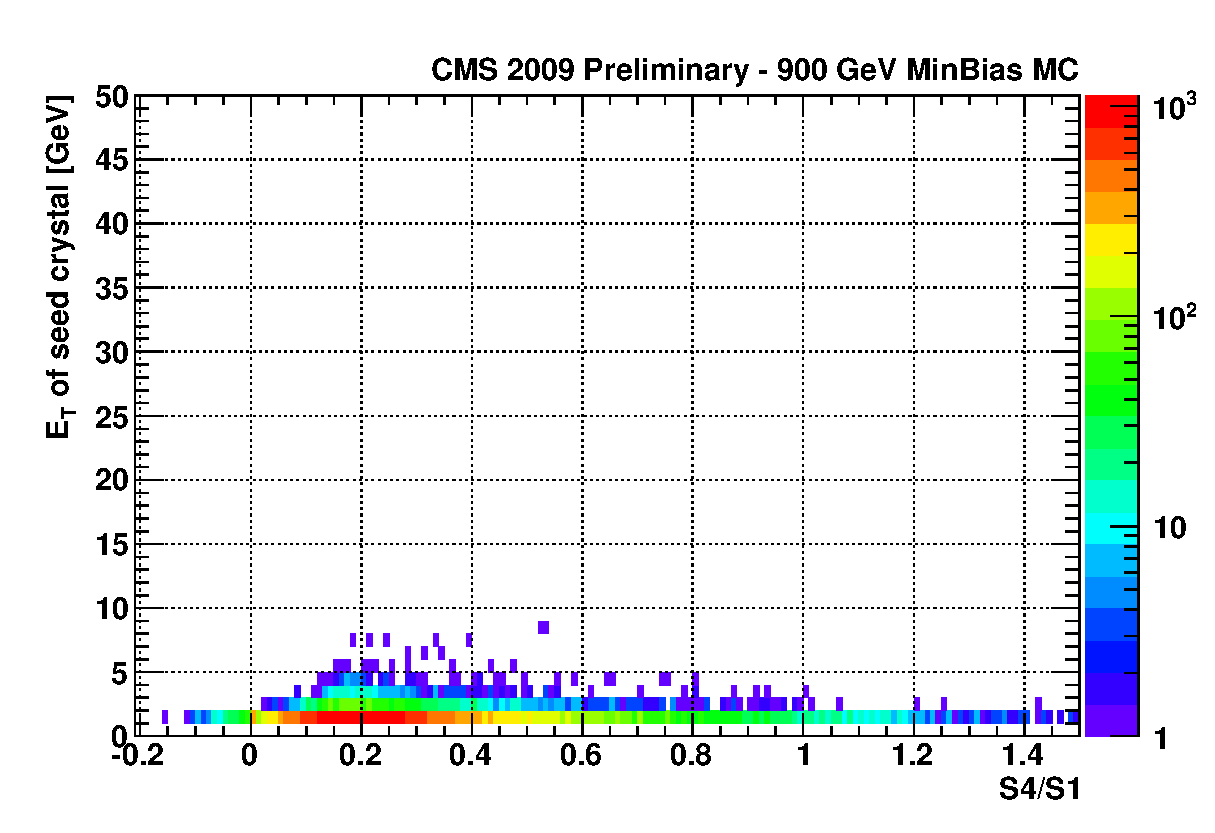
\includegraphics[width=0.5\textwidth]{plots_ecalnoise/ECalSeedET_Vs_S4_MC900GeV.eps}\\
 \end{tabular}
\caption{Distributions of the $S4/S1$ in 900 GeV data and Monte Carlo
  for barrel ECAL. Distributions are shown for events that pass all
  selections described in previous sections, except HF cleaning.}
\label{fig:ecal_noise_1}
\end{figure}

The total energy deposited in the crystals in the immediate
neighbourhood of the spike is expected to be small compared to the
energy in the spike crystal itself. Therefore, the ratio of energy
deposited in the neighbourhood of the spike crystal to the energy
measured in the spike itself is expected to be very small, provided the
occupancy in the ECAL is low. In this analysis we consider the quantity
$S4/S1$, where $S4$ is defined as a sum of energies deposited in four
crystals that share an edge with the spike, and $S1$ is the energy
measured in the spike crystal. The distributions of $S4/S1$ in data and
simulation for 900 GeV are shown in Fig.\ref{fig:ecal_noise_1}. The
``hybridSuperClusters'' algorithm was used to reconstruct the ECAL
clusters. A distinct set of events in data can be observed with $S4/S1$
values below 0.01 for events with $E_T>5$~GeV in the spike
crystal. This feature is not observed in the Monte Carlo
simulation. Therefore, we identify spike events by requiring that an
ECAL crystal has $E_T>5$~GeV and $S4/S1<0.01$.

\subsection{Removal of Cosmic and BeamHalo Events}
to be added.

\subsection{Effect of noise removal}

Tables~\ref{tab:selectionefficiency_data}, \ref{tab:selectionefficiency_mc}
summarize the number of events after each set of event selection
criteria described above, as well as their efficiencies in data and
simulation. It can be seen from 
Tab.~\ref{tab:selectionefficiency_data} that the number of events
rejected by the ECAL/HCAL noise identification algorithms described
above is relatively small. However, since this
events can create an apparent imbalance in transverse energy, which can
also populate the tails of distributions, it is crucial to identify
them. Fig.~\ref{fig:calometAfterCuts} shows how the
$\etmiss$ distribution changes after removing the events with ECAL and HCAL
noise. The algorithms described above can be seen to reject the majority of
``large'' $\etmiss$ events, including the shoulder in $\etmiss$
distribution around 16-20~GeV.
 
\begin{table}[!ht]
  \begin{center}
    \begin{tabular}{|c|c|c|c|}
      \hline
      Selection      & Number of Events  & Relative Efficiency   &
      Absolute Efficiency\\
      \hline\hline
      Trigger                            & 303277 () & 1.000 ()  &  1.000 () \\ 
      Technical Trigger Bit 0    & 264900 () & 0.873  () & 0.873  ()\\
      Good Run List                 & 196792 () & 0.743 () & 0.649 () \\
      Scraping Events Removal& 195919 () & 0.996 () & 0.646 () \\
      ECAL spikes Removal     & 195767 () & 0.999 () & 0.645 () \\
      HF PMT hits Removal      & 195404 () & 0.998 () & 0.644 ()\\  \hline
  \end{tabular}
    \caption{Number of events passing each selection criteria in the 900~GeV (2360~GeV) data and
      the efficiencies of the various selections applied.}
    \label{tab:selectionefficiency_data}
  \end{center}
\end{table}

\begin{table}[!ht]
  \begin{center}
    \begin{tabular}{|c|c|c|c|}
      \hline
      Selection      & Number of Events  & Relative Efficiency   &
      Absolute Efficiency\\
      \hline\hline
      Total events                    & 735275 () &  1.000 () & 1.000 ()         \\
      Trigger                            & 500568 () & 0.681 ()& 0.681 () \\ 
      Scraping Events Removal& 500568 () & 1.000 () & 0.681 () \\
      ECAL spikes Removal     & 500568 () & 1.000 () & 0.681 () \\ 
      HF PMT hits Removal      & 500566 () & 0.999 () & 0.681 ()\\ \hline
 \end{tabular}
    \caption{Number of events passing each selection criteria in the 900~GeV (2360~GeV) Monte Carlo samples and
      the efficiencies of the various selections applied.}
    \label{tab:selectionefficiency_mc}
  \end{center}
\end{table}

\begin{figure}[h!]
 \centering
 \begin{tabular}{ll}
  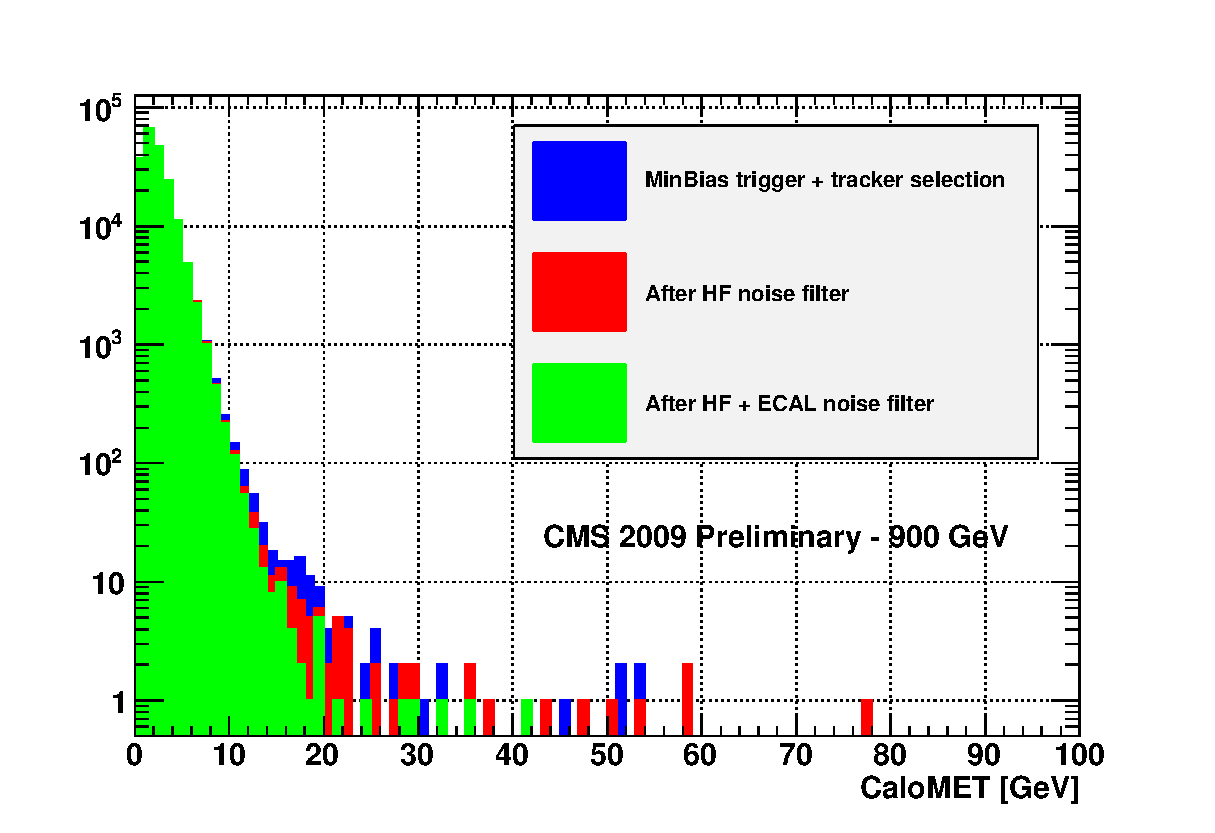
\includegraphics[width=0.5\textwidth]{plots_EventSelection/calometPt_afterFilters_900.eps} &
  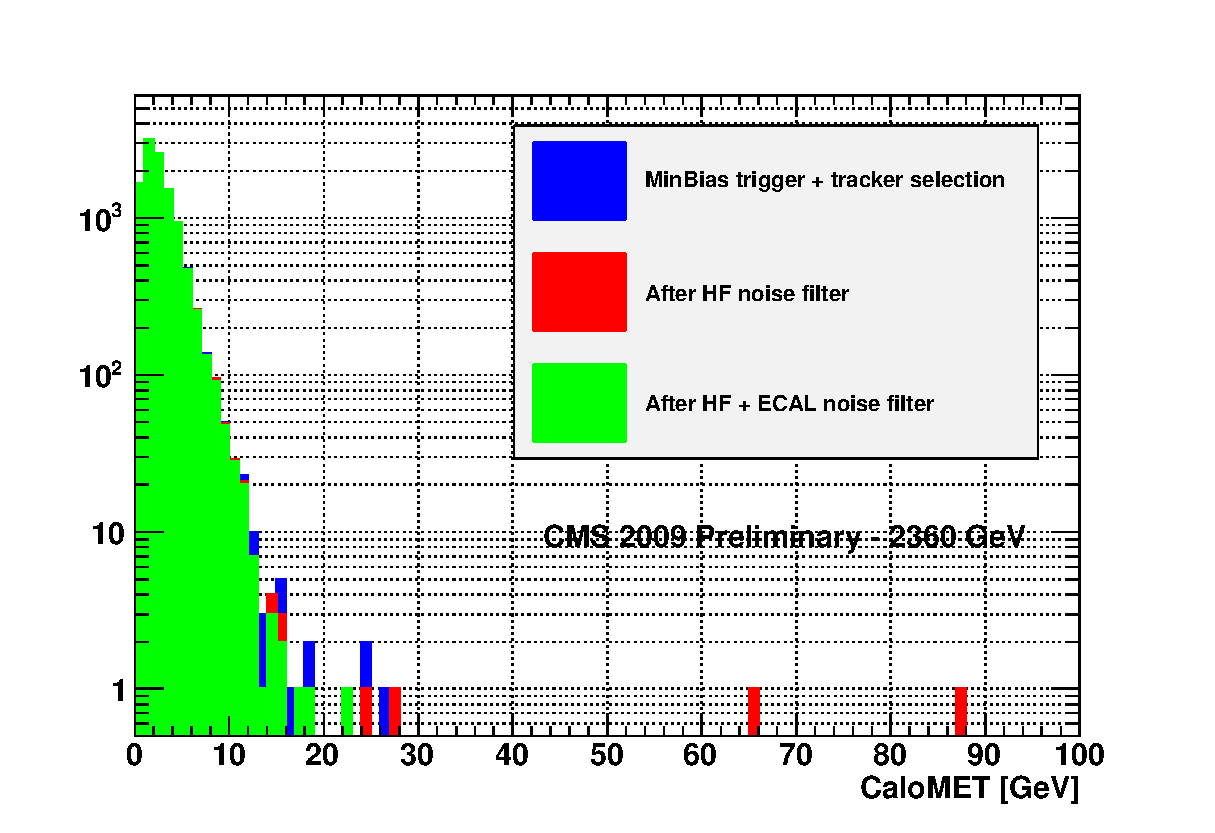
\includegraphics[width=0.5\textwidth]{plots_EventSelection/calometPt_afterFilters_2360.eps} \\
 \end{tabular}
 \caption{$\etmiss$ distributions in 900 GeV and 2360 GeV data after different levels of event selection ~\label{fig:calometAfterCuts}}
\end{figure}

\section{Effects of Machine-Induced Backgrounds}
\label{sc:BeamHalo}

The effects of machine-induced backgrounds, often referred to as beam halo, can be quite detrimental to $\etmiss$ or $\etmiss$-related quantities.  Figure~\ref{fig:BH_EventDisplay} shows a visualization of such an event, recorded during collision Run 123893~\footnote{ Run 123893 is not considered in the ``good'' run list as the Silicon Tracker was not participating in the run.}. Fortunately, lessons learned from the Tevatron experiments motivated an intense effort to identify beam halo and preclude its potential harmful effects to the $\etmiss$ observable.  To this end, several strategies and algorithms have been consolidated into a common framework known as the \verb BeamHaloId  package, which is executed during the standard reconstruction sequence as of \verb CMSSW_3_4_1 . 
  
\begin{figure}[htp]
\begin{center} 
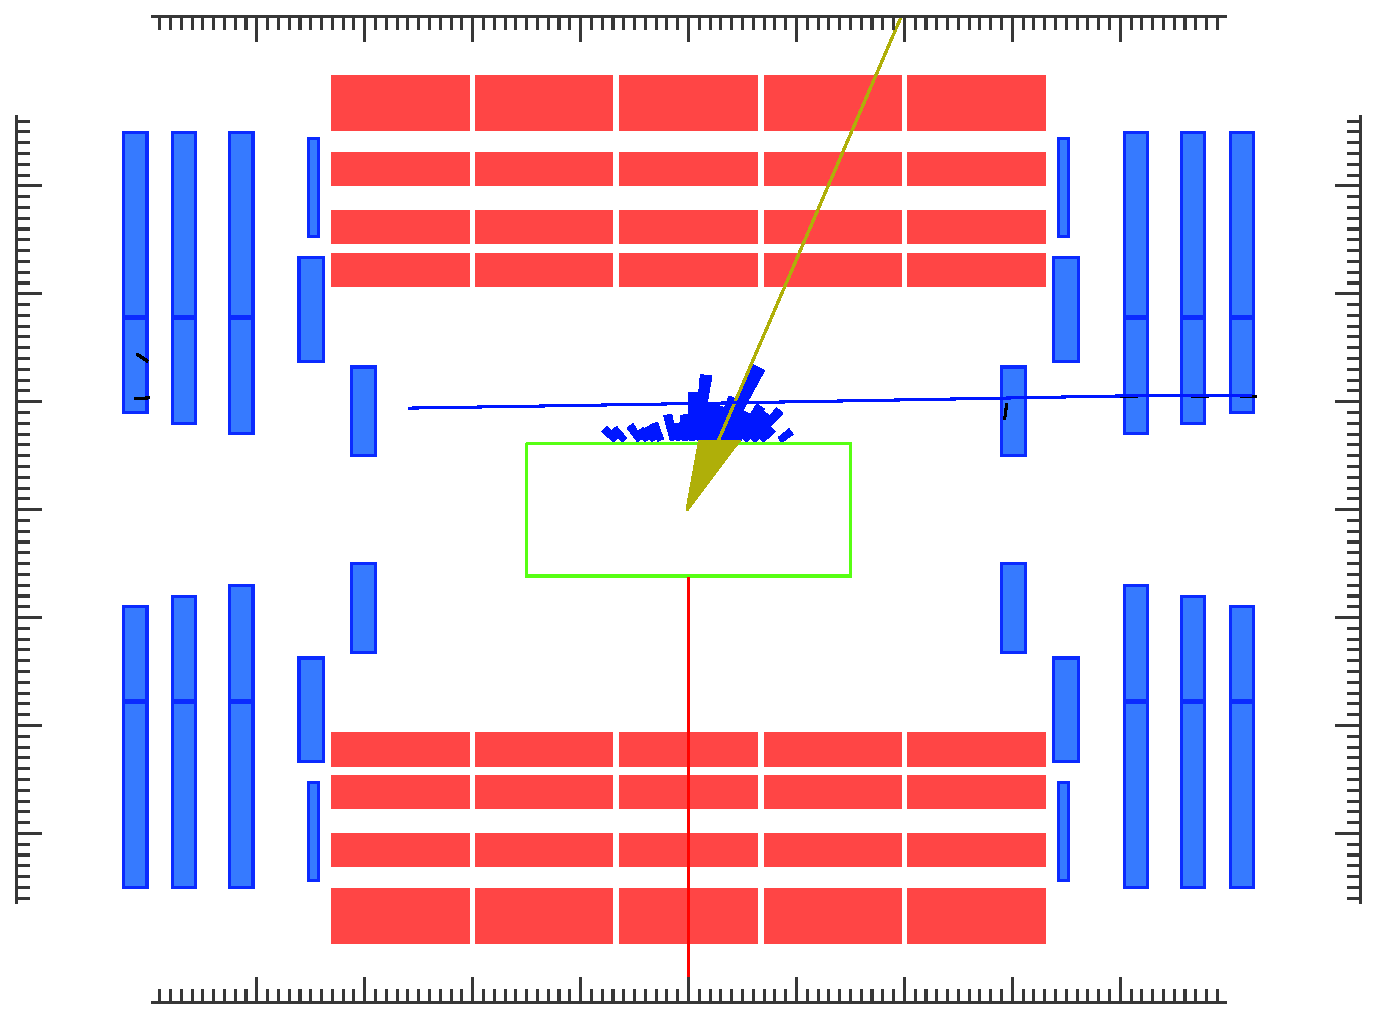
\includegraphics[scale=0.5]{plots_BeamHalo/Run123893_Lumi42_12070813_RZ.eps}
\end{center}
\caption{Event 12070813 from collision Run 123893.  Due to the kinematics of the beam halo particle, several energy deposositions are concentrated in a small $\phi$ window in the HCAL, yielding $\etmiss$ = 59.4 GeV.}
\label{fig:BH_EventDisplay}
\end{figure}

The \verb BeamHaloId  package is primarily designed to identify beam halo candidates which have trajectories pointing towards the barrel or endcap calorimetry. These are the most dangerous if one considers how the calorimeter-based $\etmiss$ overvable is constructed, i.e., via a negative vector sum over the transverse energy components of the calotowers.  Because beam halo particles are expected to have mostly parallel-to-beam trajectories, any interactions with the CMS calorimeters are very likely to occur along a narrow window in $\phi$.  Energy deposits in this pattern will conspire to maximally contaminate the magnitude of the $\etmiss$ vector, in contrast to a scenario where they are randomly distributed in $\phi$ allowing for some cancellations to occur. Of course, other MET algorithms which rely on the calorimetry are susceptible to beam halo as well.  

In order to best identify beam halo, information from three subdetectors is used in both a stand-alone and global way. In the Ecal and Hcal topological signatures, as well as time-of-flight information,  are used to identify halo at the rechit level.  The granularity of the Ecal also allows for observables based on showershapes to be employed in the identification of beam halo.  This information from the calorimeters is combined with information from the CSCs to identify halo in a global way, as the CSCs are extremely efficient at measuring muons, both collsion and beam-induced.  If the halo particles are charged, they will likely be measured by the CSCs in route to the calorimeters, as the CSCs provide nearly full geometrical coverage of barrel and endcap calorimetry in the transverse plane. There is even a dedicated Level-1 beam halo trigger implemented in the CSC Track Finder.  This trigger exploits the basic kinematic features of beamhalo, imposing a tight $\delta$($\phi$) window and a minimum $\delta$($\eta$) requirement on two LCTs (local charged tracks) in stations 1 and 2 or 1 and 3. The details of this trigger can be found in CMS IN-2008/041, by D. Acosta, et al.

In order to commission the \verb BeamHaloId  tools in data, a pure sample with high statistics is needed. The CSC beam halo trigger is very useful for this purpose.  Unfortunately, mainy of the Single-Beam Commissioning runs of 2009 did not feature CSC station ME1/1, which is the station closest to both the calorimeters and the beam line. This station is anticipated to get the most halo flux, but was often kept in standby mode in order to safeguard the hardware and electronics from beam splash events.  As a result, not many genuine beam halo events were triggered. Nonetheless, a small amount of events were gleaned from the collision runs via the CSC beam halo trigger.  Because the cosmic background contamination to the CSC beam halo trigger is about 0.6 Hz, a requirement on the BPTX technical trigger was also imposed.  Given that there are 3564 possible bunch crossings (or spacings) per orbit, the rate for a cosmic to fake a CSC beam halo trigger and coincide with BPTX trigger bit 0, can be estimated as:

\begin{eqnarray}
R_{fake} = \frac{(0.6Hz)\times N_{BX}}{3564}
\end{eqnarray}
where $N_{BX}$ represents the number of filled, colliding bunches per orbit. It is assumed the BPTX trigger bit 0 operates with 100\% efficiency.  This fake rate becomes $1.64 \times 10^{-4}$Hz , $3.28 \times 10^{-4}$ Hz, $4.93 \times 10^{-4}$ Hz for 1, 2, and 3 colliding bunches per orbit respectively. 
  
Table~\ref{tab:BHStats} gives the beam halo statistics for each good collision run. Because only a filled bucket from one beam is necessary to produce beam halo, all BPTX technical triggers corresponding to single-beam filled buckets were considered.  The subset of events with BPTX technical trigger bit 0 are also given so that one can calculate the probability for beam halo overlap with a minbias event.  For most of the earlier runs, the rates calculated are consistent with the cosmic background.  For the later runs, the rates are higher by roughly an order of magnitude, which indicates the unmbiguous presence of machine-induced backgrounds.    \\
     
\begin{table}[h]
\begin{center}
\begin{tabular}{|c|c|c|c|c|c|c|} \hline
        &       &       & \multicolumn{4}{|c|}{L1\_SingleMuBeamHalo} \\ \hline
        &       &       & \multicolumn{2}{|c|}{ \&\& BPTX Bits 0-6 }  & \multicolumn{2}{|c|}{\&\& BPTX Bit 0}      \\ \hline
 Run    & Colliding BXs & Lumis &  Events & Rate [Hz] &  Events & Rate [Hz] \\ \hline 
123596  &  2  & 144& 1   & 7.5e-05  & 1  & 7.5e-05 \\ \hline 
123615  &  2  & 26 & 1   & 2.0e-04  & 1  & 2.0e-04 \\ \hline 
123815  &  2  & 9  & 4   & 2.4e-03  & 4  & 2.4e-03 \\ \hline 
123818  &  2  & 41 & 3   & 7.2e-04  & 2  & 4.8e-04 \\ \hline 
123906  &  1  & 23 & 0   & --       & 0  & -- \\ \hline 
123908  &  1  & 27 & 2   & 7.9e-04  & 2  & 7.9e-04 \\ \hline 
123909  &  1  & 28 & 10  & 3.8e-03  & 10 & 3.8e-03 \\ \hline 
124008  &  3  & 2  & 0   & --       & 0  & -- \\ \hline 
124009  &  3  & 68 & 28  & 4.4e-03  & 23   & 4.4e-03 \\ \hline 
124020  &  3  & 98 & 21  & 2.3e-03  & 18   & 2.0e-03 \\ \hline 
124022  &  3  & 152& 54  & 3.8e-03  & 48   & 3.4e-03 \\ \hline 
124023  &  3  & 89 & 38  & 4.6e-03  & 35   & 4.2e-03 \\ \hline 
124024  &  3  & 81 & 30  & 4.0e-03  & 26   & 3.4e-03 \\ \hline 
124025  &  3  & 13 & 2   & 1.7e-03  &  2   & 1.7e-03 \\ \hline 
124027  &  3  & 35 & 24  & 7.4e-03  & 20   & 6.1e-03 \\ \hline 
124030  &  3  & 31 & 12  & 4.2e-03  & 11   & 3.8e-03 \\ \hline 
124120* &  1  & 57 & 51  & 9.6e-03  & 45   & 9.6e-03 \\ \hline 
%Totals  &  1  & 73 & 12  & 1.8e-03  & 12   & 1.8e-03 \\ \hline 
%        &  2  & 220& 9   & 4.4e-04  & 11   & 3.9e-04 \\ \hline
%        &  3  & 567& 209 & 4.0e-03  & 183  & 3.5e-03 \\ \hline
%\multicolumn{2}{|c|}{Total}  & 902 (57) & 231 (51) &  -- & 202 (45) & -- \\ \hline    
%\multicolumn{2}{|c|}{Total}  & 902 (57) & 231 (51) & 2.7e-03 (9.6e-03) & 202 (45) & 2.4e-03  \\ \hline    
\end{tabular}
\end{center}
\caption{Summary of beam halo statistics for good collision runs at $\sqrt{s}=900$~GeV ($2.36$~TeV). *Run 124120 featured $\sqrt{s}=2.36$~TeV. A lumisection is included if it features BPTX bit 0 operating at nominal rates (indicating both beams crossing) and the L1\_SinglMuBeamHalo trigger operating at a minimum of the cosmic rate (indicating the CSCs and Track Finder are active)}
\label{tab:BHStats}
\end{table}

With these limited statistics some meaningful distributions can still be made. Figure~\ref{fig:BH_CaloMET} shows the differential  CaloMET rate for these selected events.  A few events exist beyond $\etmiss \ge 10$ GeV, which implies that some halo muons are hitting the calorimeters. Figures~\ref{fig:BH_Radial} and~\ref{fig:BH_Phi} show the position of the halo muon in the CSCs at its point of closest approach with respect to the calorimeters.  This information is extracted from the innermost rechit from the  CSC stand-alone cosmic track (if there was one reconstructed in the event).  The cosmic track reconstruction algorithms are optimized to measure muons which do not come from the collision point.

Of these 281 events, 261 or 92.8\% had at least one~\footnote{In some cases the halo muon will leave enough hits in both plus and minus muon endcaps to allow for two separate tracks to be reconstructed.} CSC stand-alone cosmic track in them, while 18 or 6.4\% had segments.  One event had no track or segments, but had rechits in the CSCs, and one event had no reconstruction level activity at all in the CSCs, despite the existence of a L1 CSC beam halo trigger.  The events in the CaloMET tails in Fig~\ref{fig:BH_CaloMET} all had stand-alone cosmic tracks in them.  

It will be important to measure and monitor these rates once the beam intensities increase along with the frequency of minbias events. The probability of contamination is negligible in the current set of collision runs.  None of these events with CSC beam halo triggers survive the standard event selection beyond the BSC requirements. This may not be the case, however, in the future.  \\


\begin{figure}[htp]
\begin{center}
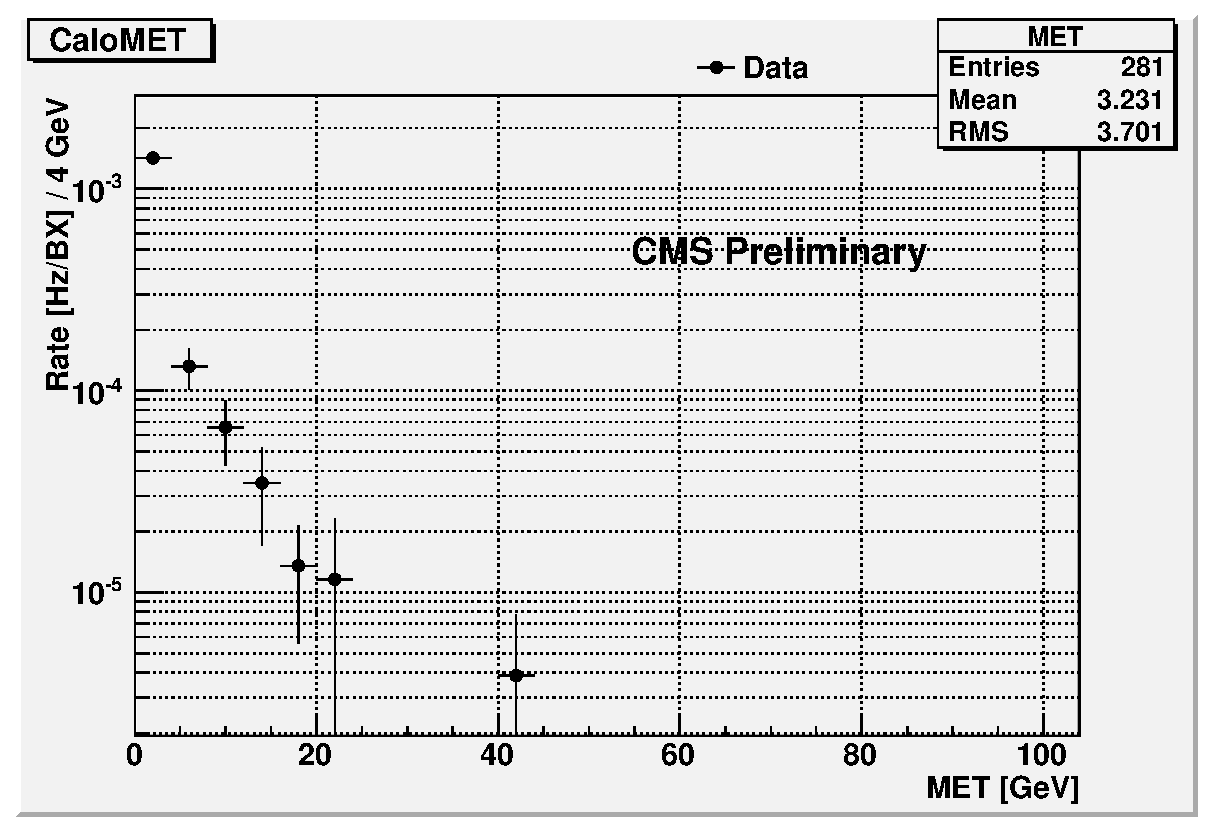
\includegraphics[scale=0.75]{plots_BeamHalo/CaloMET.eps}
\end{center}
\caption{$\etmiss$ differential rate distribution from the CSC beam halo AND BPTX triggered events recorded during the collision runs. Statistics were combined from each good collision run, including Run 124120 (2.36 TeV), and rates are normalized to a single bunch crossing.   }
\label{fig:BH_CaloMET}
\end{figure}

\begin{figure}[htp]
  \begin{center}
    \subfigure[Radial distribution of CSC halo tracks' impact point]{\label{fig:BH_Radial}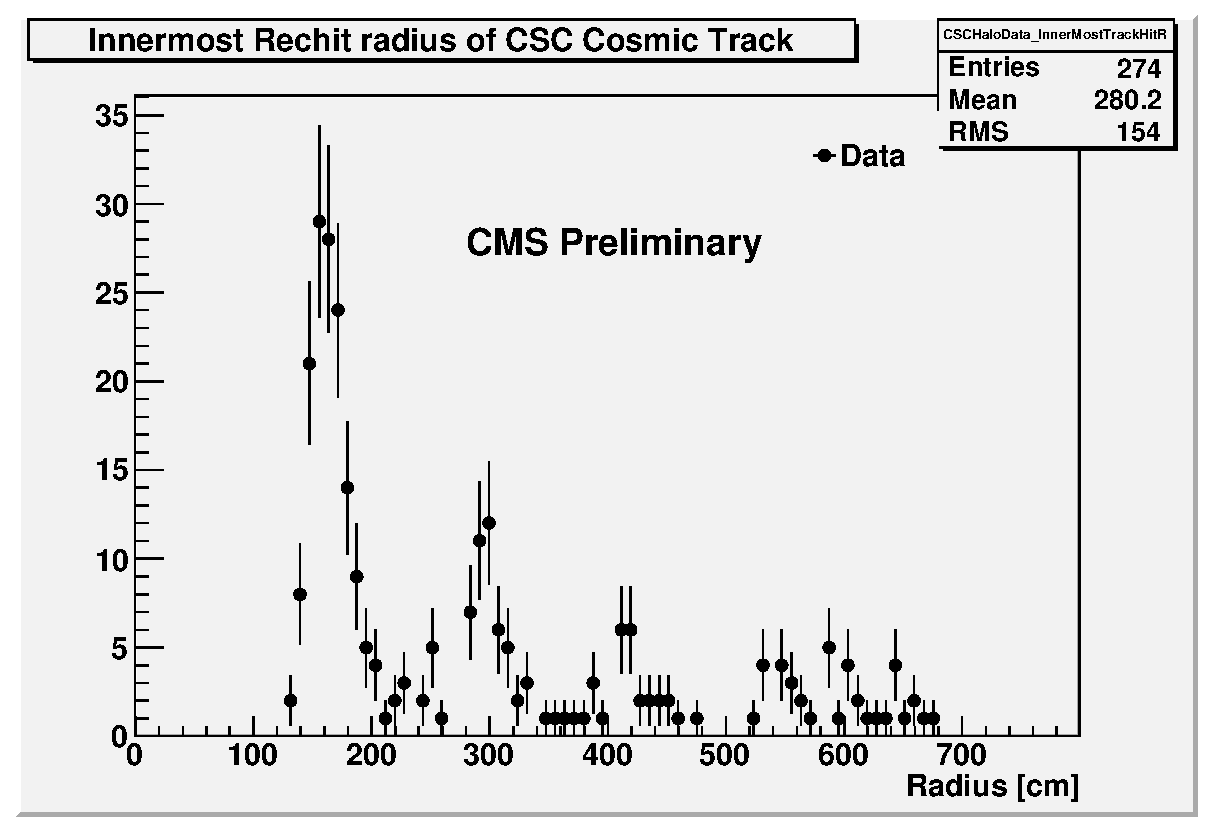
\includegraphics[scale=0.65]{plots_BeamHalo/InnerMostTrackHitR.eps}}
    \subfigure[$\phi$ distribution of CSC halo tracks' impact point]{\label{fig:BH_Phi}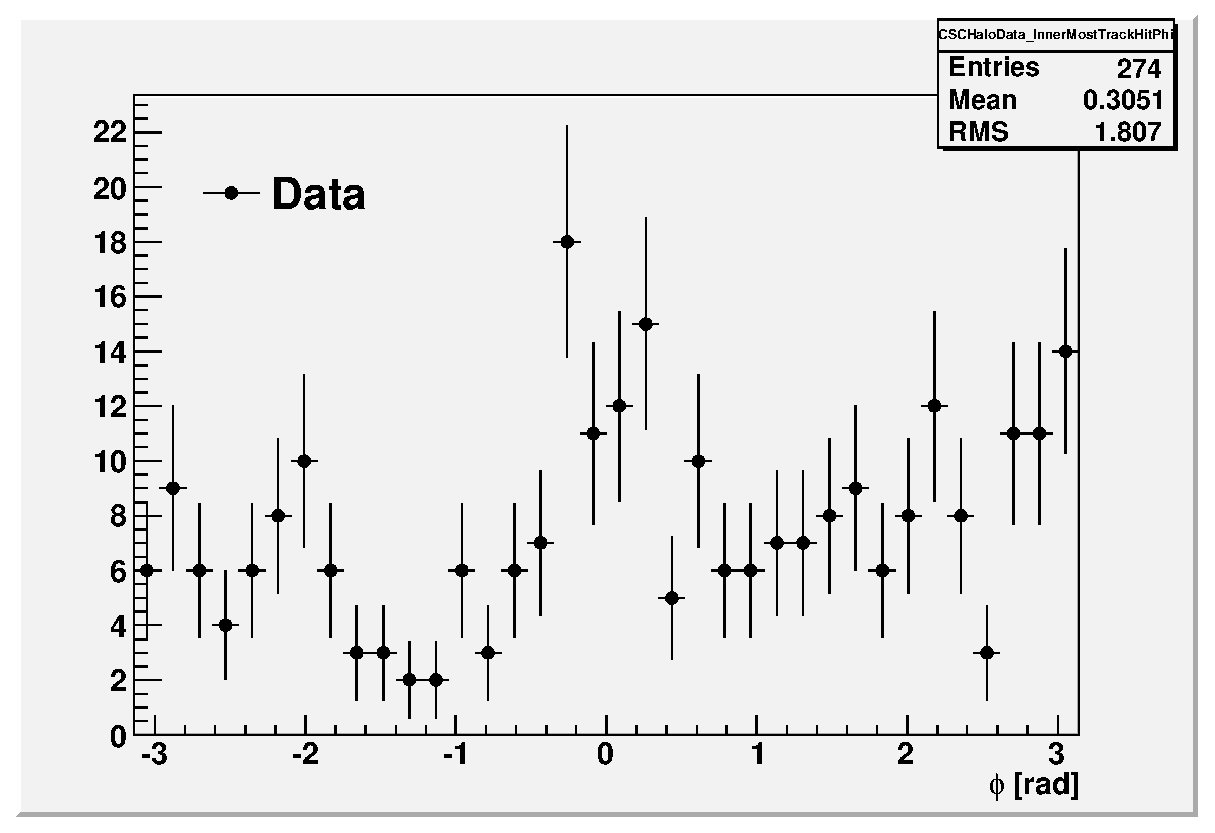
\includegraphics[scale=0.65]{plots_BeamHalo/InnerMostTrackHitPhi.eps}}
    \end{center}
  \caption{Global position of the constituent rechit of CSC stand-alone cosmic tracks at point of closest approach with respect to the calorimetry. Note: the  ECAL Barrel spans a radius from roughly 140 cm to 190 cm, while the Hcal Barrel spans roughly from 200 cm to 300 cm. The beam halo flux is expected to decrease as a function of radius. } 
  \label{fig:BH_ImpactPoint}
\end{figure}




\clearpage

